\section{Introduction}
\label{sec:introduction}

A common goal in reliability engineering is to understand when and how a system fails.
%
In a simulation setting, this means understanding where in the simulation input space the system transitions from normal operation to a failure case.
%
When taken collectively over the input space, this area of transition is known as the limit surface, or decision boundary, and can be thought of as a (hyper)surface or collection of (hyper)surfaces dividing the domain into regions of normal function and regions of failure.
%
A better understanding of the global/local shape and gradient of the limit surface can inform practitioners of the stability of the system under study.
%
With this information, practitioners can build surrogate models that best exploit local behaviors of the limit surface and/or report on the confidence of constructed models.
%
As an example, understanding the complexity or lack thereof attached to a limit surface can influence a model builder to either collect more samples or construct their model with the current collected data.
%
For instance, one may be tempted in a high-dimensional problem to generate a larger number of samples than for a two-dimensional problem, but if the limit surface for the two dimensional problem consists of several disjoint components or has a highly convoluted shape, it may take more samples to resolve than a hyperplane limit surface in the higher-dimensional space.
%
In addition, a more complex limit surface may indicate that a simulation is better modeled by using multiple, local surrogates rather than a global surrogate.

In this work, we investigate methods for estimating limit surfaces in arbitrary dimensional spaces given a limited set of observed training samples.
%
The goal of this work is to apply the lessons learned to a simulation of a multi-unit nuclear power plant consisting of six distinct possible failure components.
%
Simulating the success/failure of each of the six components stems from a collection of computationally intensive simulations, and therefore the scientists studying this system seek to utilize more efficient surrogate models to represent each of the six components in order to generate enough samples for further analysis.
%
We briefly discuss the construction and use of the resulting surrogate models, however the main focus of this paper is to evaluate the sampling of the input space and reliability of the constructed surrogate models by analyzing the limit surfaces extracted from each training sample set.

% test citation~\cite{Nureg1150} and test figure~\ref{fig:raven}

% \begin{figure}
%     \centering
%     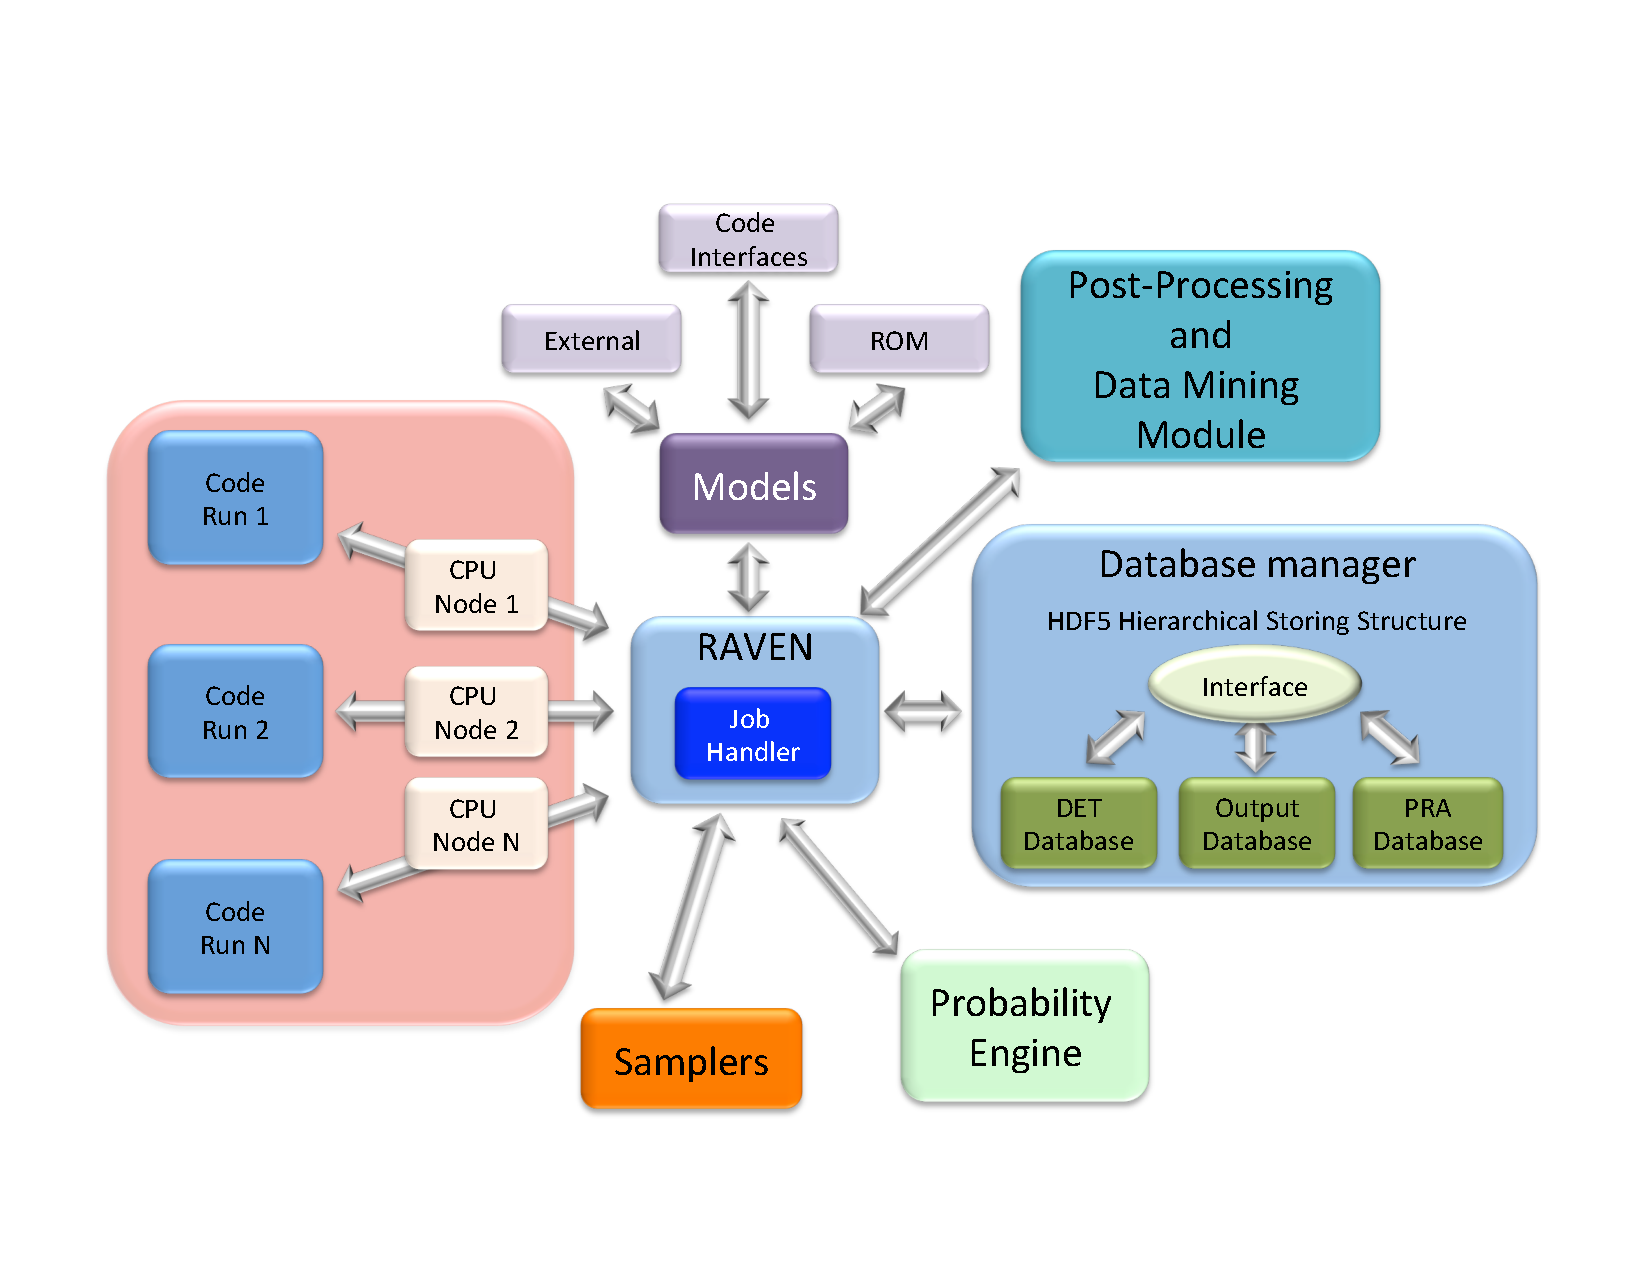
\includegraphics[scale=0.5]{raven.pdf}
%     \caption{RAVEN}
%     \label{fig:raven}
% \end{figure}
